\section{Introduction to Boosting}
%
\begin{frame}
  Boosting encompasses a highly successful set of learning algorithms.
  
  \begin{itemize}
    \item Allstate has held three Kaggle competitions.  All three were won by algorithms incorporating gradient boosting as a fundamental component.
    \item In the 1990's the insurance industry discovered that incorporating consumers credit information into pricing greatly increased the accuracy of prices, this revolutionized the industry.  Using a boosted model in place of a linear model when setting prices gives roughly the same increase in power.
  \end{itemize}
\end{frame}
%
\begin{frame}
Boosting can adapt itself effortlessly to very non-linear objectives
  \only<1>{
    \begin{figure}
      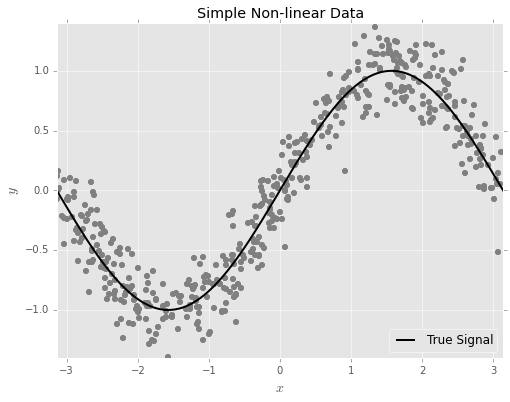
\includegraphics[scale=0.50]{sin-with-data}
    \end{figure}
   }
   \only<2>{
    \begin{figure}
      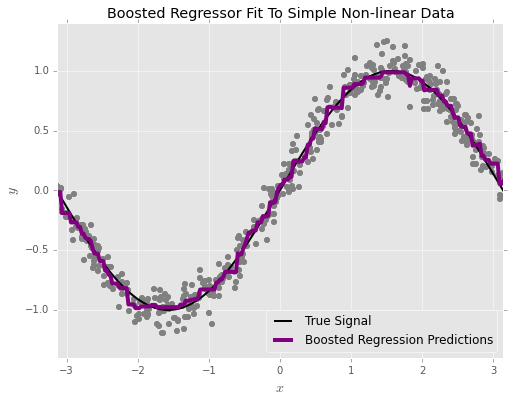
\includegraphics[scale=0.50]{sin-with-data-and-booster}
    \end{figure}
   }
   \only<3>{
    \begin{figure}
      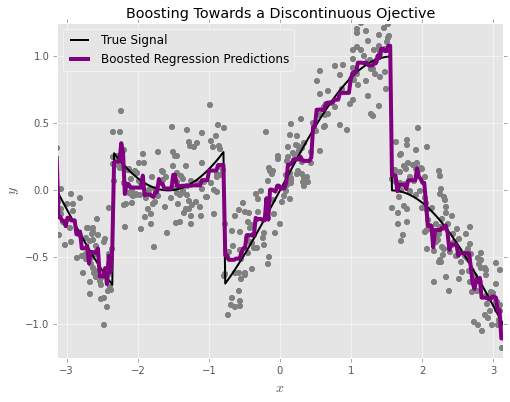
\includegraphics[scale=0.50]{broken-sin-with-booster}
    \end{figure}
   }
\end{frame}
%
\begin{frame}
Boosting accomplishes this by \textit{growing the model gradually}
  \begin{figure}
    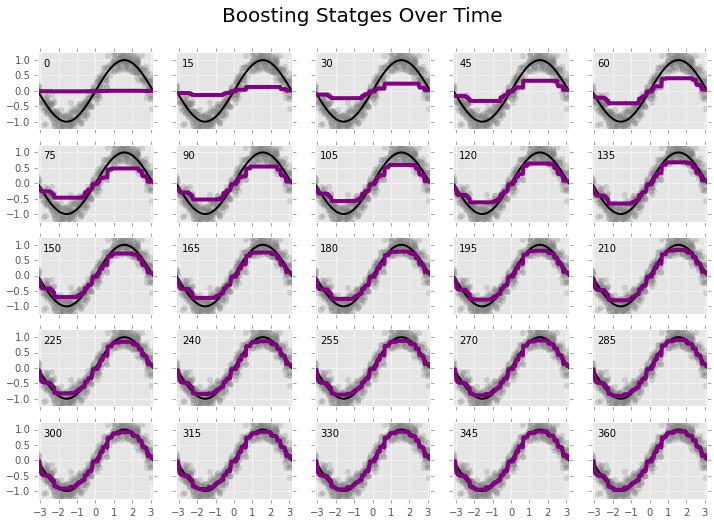
\includegraphics[scale=0.40]{boosting-over-time-multiple-plots}
  \end{figure}
\end{frame}
%
\begin{frame}
At each stage of the growth, the next model is built as an adjustment to the previous model
  \begin{figure}
    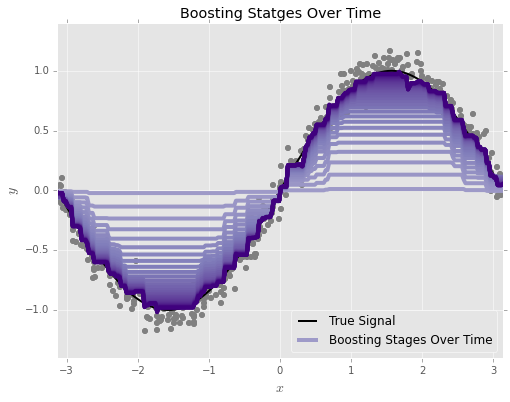
\includegraphics[scale=0.50]{boosting-over-time-single-plot}
  \end{figure}
\end{frame}